\section{Tassonomia definita in letteratura}
\subsection{Risultati Preliminari}
Lo studio ha riportato dalla collezione per ogni sorgente un'insieme iniziale di 156 articoli, di cui:
\begin{itemize}
    \item 89 articoli provenienti da \textit{Scopus},
    \item 1 articolo proveniente da \textit{IEEEXplore Digital Library},
    \item 21 articoli provenienti da \textit{ACM Digital Library},
    \item 45 articoli provenienti da \textit{Web of Science}.
\end{itemize}
Dalla collezione poi è stata effettuata una rimozione degli articoli duplicati, per giungere a un totale di 80 articoli.
In seguito al processo di revisione manuale di titolo e abstract per ogni articolo tramite l'utilizzo dei criteri di inclusione e di esclusione, 66 articoli sono stati esclusi dai revisori.
In particolare, durante l'analisi preliminare condotta su titolo e abstract dell'articolo, 
9 articoli su 80 sono stati accettati da entrambi i revisori.
Il numero di articoli che hanno ricevuto una valutazione in conflitto sono 8.
I revisori che hanno svolto il ruolo di terzo revisore hanno accettato 5 articoli su 8, avendo come risultato dell'analisi preliminare un totale di 14 articoli.
Inoltre, i risultati del processo di revisione manuale completo hanno portato all'esclusione di altri 8 articoli di ricerca.
Quindi per il primo ciclo di analisi sono stati ritrovati infine 6 articoli di ricerca.
Per estendere i risultati è stato deciso di applicare la tecnica di \textit{backward snowballing} \cite{WohlinSnowballing}.
 Questa tecnica permettere di utilizzare la lista di referenze di ogni articolo per identificare nuovi articoli da includere.
 Il primo passaggio prevede quindi, attraverso l'analisi della lista delle referenze, l'esclusione degli articoli tramite l'utilizzo dei criteri di esclusione.
 Successivamente, si escludono i paper che sono stati già esaminati durante il processo di review. Infine, si riattiva il processo di review per gli articoli che non sono stati esclusi.
 Attraverso l'utilizzo dello snowballing, altri 2 articoli sono stati accettati dal processo di review e inclusi.
 Il processo di revisione della letteratura, quindi, ha come risultato l'estrazione di 8 articoli.
 
 La distribuzione dei paper selezionati sugli anni di pubblicazione è mostrata in Figura \ref{fig:year_chart}.
 Sulla asse delle X è rappresentata la serie degli anni di pubblicazione, mentre sulla asse delle Y è rappresentato il numero di articoli per ogni anno.
 Dal grafico è possibile notare che a partire da una pubblicazione iniziale risalente al 2015, l'interesse da parte dei ricercato è aumentato negli ultimi anni, ritrovando 7 articoli di ricerca pubblicati negli ultimi 4 anni.
 
 \begin{figure}[h]
     \centering
     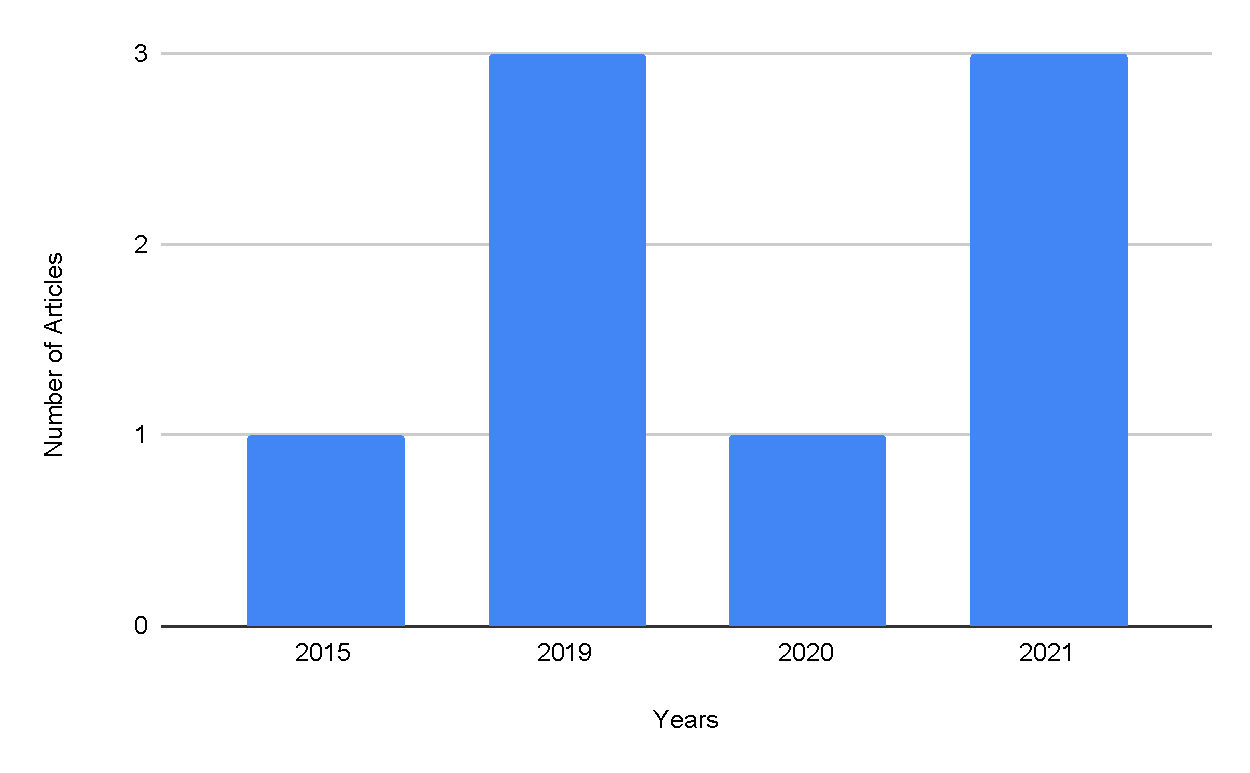
\includegraphics[width=\textwidth]{Figure/Results/SLRResults/year_chart.pdf}
     \caption{Distribuzione degli articoli per anno di pubblicazione}
     \label{fig:year_chart}
 \end{figure}

Tra gli articoli selezionati in questa ricerca ritroviamo 7 articoli che sono che sono stati pubblicati a conferenze internazionali e 1 articolo pubblicato a un workshop. 
In particolare, tra gli articoli pubblicati alle conferenze ritroviamo 1 articolo pubblicato alla "International Conference on Product-Focused Software Process Improvement" (PROFES), 1 articolo pubblicato alla "International Conference on Technical Debt" (TechDebt) e 2 articoli pubblicati alla "International Conference of Software Engineering" (ICSE). 
Questi articoli sono stati pubblicati tutti in conferenze relative all'ingegneria del software, dimostrando quindi che la ricerca relativa all'investigazione di AI Technical Debt ha generato significativo interesse nella comunità di ricerca di ingegneria del software. La lista degli articoli analizzati per questa Systematic Literature review è disponibile nel replication package in \cite{slr_rp}.

\subsection{RQ1.1: Quali tipologie di AITechnical Debt sono presenti in letteratura?}
La Figura \ref{fig:slr_td_type} mostra la distributzione di referenze delle tipologie di AITechnicalDebt nella letteratura.
E' possibile notare come \textit{Data Debt} sia estremamente di riferimento per gli articoli che trattano pratiche di ingegneria del software per i sistemi di intelligenza artificiale, in quanto 5 articoli su 8 trattano questa tipologia di AITechnicalDebt.
Successivamente, con un alto tasso di riferimento, ritroviamo \textit{Configuration Debt}, \textit{Code Debt} e \textit{Architectural Debt}.

\begin{figure}[h!]
    \includegraphics[width=\textwidth]{Figure/Results/SLRResults/RQ1.1/debt_type_count.pdf}
    \caption{Tipologie di AI Technical Debt riscontrate in letteratura}
    \label{fig:slr_td_type}
\end{figure}

In particolare, la Figura \ref{fig:slr_td_instances} mostra la distribuzione di referenze nella letteratura per ogni articolo di ricerca. L'istanza di AI Technical Debt ritrovata maggiormente in letteratura è l'istanza di \textit{Pipeline Jungle}, ritrovando 4 articoli su 8 in letteratura che trattano dei danni che può apportare al sistema AI un incremento smisurato e incontrollato della pipeline AI.
Successivamente, molte istanze di AI Technical Debt sono presenti.
Unstable Data Dependencies, Bundled Features, Correlated Features, Epsilon Features e Feature Entanglement sono le istanze di AI Data Debt che sono state ritrovate, dimostrando l'interesse attuale della ricerca nel trovare metodologie e tecniche utili a preservare la qualità dei dati.

\begin{figure}[h!]
    \includegraphics[width=\textwidth]{Figure/Results/SLRResults/RQ1.1/debt_instance_count.pdf}
    \caption{Istanze di AI Technical Debt riscontrate in letteratura}
    \label{fig:slr_td_instances}
\end{figure}

Analizzando le istanze e le tipologie ritrovate, è possibile conseguire che c'è un'alto interesse della ricerca nell'investire lo sforzo al fine di migliorare le metodologie attuali per preservare la qualità e l'elaborazione dei dati.
Tuttavia, la ricerca ritiene di alto interesse anche gli aspetti architetturali e del codice del sistema AI, riscontrando un alto tasso di interesse rispettivamente per \textit{Pipeline Jungles}, \textit{Glue Code}, e \textit{Multiple Language Smell}.

\subsection{RQ1.2: Quali sono gli approcci di identificazione e mitigazione di AI Technical Debt?}

Sebbene esiste una definizione per le diverse tipologie e istanze di AI Technical Debt, diverso è per le loro tecniche di identificazione e mitigazione.
Possibili spiegazioni estratte dagli articoli in letteratura sono : 
\begin{itemize}
    \item Il codice relativo al modello contiene la minor quantità di codice di tutto il sistema [S01].
    \item I professionisti di data science potenzialmente concentrano i loro al fine di massimizzare le performance del modello, piuttosto che la manutenzione e l'evoluzione del codice AI [S02].
\end{itemize}
Il nostro studio ha riportato come output una singola tecnica di identificazione per la presenza di \textit{Epsilon Feature} all'interno del sistema AI.
La tecnica estratta dalla letteratura è nominata \textit{Leave-One-out Feature Evaluation}.
Si consideri un insieme di feature $F=(f_1,f_2,...,f_n)$ dove con $f_i$ si rappresenta la feature nella struttura dei dati in posizione $i$.
Si estrae e si calcola l'insieme $(F-f_i)$ dove consideriamo l'insieme delle feature rappresentate sottratto da una particolare feature.
Vengono costruiti quindi due modelli $M$ e $M_i$ sui due insieme definiti.
Se la differenza delle performance risultanti dai due modelli non è significativa, significa che il modello $M$ conteneva una particolare istanza di \textit{Epsilon Feature} rappresentata da $f_i$.
Il processo viene poi eseguito ciclicamente per ogni $f_i$ appartenente a $F$.\\


\keyfindingsrqa{
L'interesse della ricerca è focalizzato sullo studio delle istanze di AI Technical Debt relative ai data (data debt), in particolare sulla diffusione e sulla severità di istanze relative alla presenza di dipendenze instabili tra i dati.
Inoltre, un consistente sforzo della ricerca è impuntato verso le istanze di AI Technical Debt incentrate sul codice (code debt), sulla configurazione (configuration debt) e sull'architettura (architectural debt). 
}

